\section{Markov Random Fields}
\subsection{Intuition}
We saw previously that we cannot draw a \textit{perfect} I-map such that $\mathcal I(\mathcal G) = \mathcal{I}(P)$ for any distribution $P$ using directed graphical models. Such too is the case with undirected graphical models, but they help us to represent some of these independencies which directed graphs couldn't.\\
To be added.

\subsection{Cliques}
\begin{defn}[Complete Graph]
A complete graph is a simple undirected graph in which every pair of distinct vertices is connected by a unique edge.
\end{defn}

\begin{defn}[Clique]
A clique $C$ in an undirected graph $G = (V,E)$ is a subset of vertices, $C\subseteq V$ such that every two distinct vertices are adjacent. Thus, the subgraph induced by $C$, i.e $G\braket{C}$, is a complete graph.
\end{defn}

\begin{defn}[Maximal Clique]
A clique that cannot be extended by including one more adjacent vertex (i.e it does not exist exclusively within the vertex set of a larger clique) is a maximal clique.		
\end{defn}

\begin{defn}[Maximum Clique]
A maximum clique of a graph $G$, is a clique such that there is no other clique with more vertices.
\end{defn}
With each clique $C$, we associate a potential function $\psi$, which is a provisional function of its arguments that assigns a pre-probabilistic score of their joint distribution. It is to note that $\psi$ must be non-negative, but it shouldn't be interpreted as probability. 

\subsection{Gibbs Fields}
\begin{marginfigure}
\centering
\begin{tikzpicture}[main/.style = {draw, circle}] 
	\node[main] (a) {$x_1$}; 
	\node[main] (c) [right of=a] {$x_3$}; 
	\node[main] (e) [right of=c] {$x_5$}; 
	\node[main] (b) [below = of $(a)!0.5!(c)$] {$x_2$};
	\node[main] (d) [below = of $(c)!0.5!(e)$] {$x_4$};
	\draw[-] (a) -- (c);
	\draw[-] (c) -- (e);
	\draw[-] (c) -- (b);
	\draw[-] (c) -- (d);
	\draw[-] (a) -- (b);
	\draw[-] (d) -- (e);
\end{tikzpicture}
\caption{A Gibbs Field}
\label{fig:gibbs-field-ex}
\end{marginfigure}
A Gibbs Field is a representation of a set of random variables and their relationships. An example is in Figure \ref{fig:gibbs-field-ex}. In this, the edges are undirected and imply some correlation between the connected nodes. \\
Consider clique potentials as $\psi_i(c_i)$. Then the joint probability for any set of random variables $\mathcal{X} = \{x_1, \cdots, x_n\}$ represented by a Gibbs Field can be written as a product of clique potentials
\begin{equation}
P(\mathcal X) = \dfrac{1}{Z} \prod_{c_i \in C} \psi_i(c_i)
\end{equation}
$Z$ is a normalizing constant required to create a valid probability distribution, i.e
\begin{equation}
Z = \sum_x \prod_{c_i \in C}\psi_i(C_i)
\end{equation}
\begin{rem}
For any Gibbs Field, there is a subset $\hat{C}$ of $C$ consisting of only maximal cliques, which are not proper subsets of any other cliques. We write the potentials for these maximal cliques as products of all potentials of their sub-cliques, and thus state the joint probability as
\begin{equation}
	P(\mathcal X) = \dfrac{1}{Z}\prod_{c_i \in \hat C} \hat{\psi}_i(c_i)
\end{equation}
\end{rem}
\subsection{Formal Definition}
\begin{defn}[Markov Random Field]
	A Markov Random Field (MRF) is a probability distribution $P$ over variables $x_1, \cdots, x_n$ defined by an undirected graph $G$ in which nodes correspond to variables $x_i$ and has the form
	\begin{equation}
		P(x_1, x_2, \cdots, x_n) = \dfrac{1}{Z}\prod_{c \in C} \psi_c(x_c)
	\end{equation}
	where 
	\begin{equation}
		Z = \sum_{x_1, \cdots, x_n}\prod_{c \in C} \psi_c (x_c)
	\end{equation}
	is the \textbf{\textit{partition function}} which is the normalizing constant ensuring the distribution sums to 1.
\end{defn}
\begin{marginfigure}
\centering
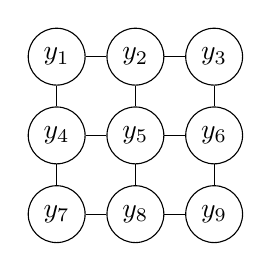
\begin{tikzpicture}[main/.style = {draw, circle}] 
	\node[main] (1) {$y_1$}; 
	\node[main] (2) [right of=1] {$y_2$}; 
	\node[main] (3) [right of=2] {$y_3$}; 
	\node[main] (4) [below of=1] {$y_4$}; 
	\node[main] (5) [right of=4] {$y_5$}; 
	\node[main] (6) [right of=5] {$y_6$}; 
	\node[main] (7) [below of=4] {$y_7$}; 
	\node[main] (8) [right of=7] {$y_8$}; 
	\node[main] (9) [right of=8] {$y_9$}; 
	\draw[-] (1) -- (2);
	\draw[-] (2) -- (3);
	\draw[-] (1) -- (4);
	\draw[-] (4) -- (5);
	\draw[-] (5) -- (6);
	\draw[-] (2) -- (5);
	\draw[-] (3) -- (6);
	\draw[-] (7) -- (8);
	\draw[-] (8) -- (9);
	\draw[-] (4) -- (7);
	\draw[-] (5) -- (8);
	\draw[-] (6) -- (9);
\end{tikzpicture}
\caption{Relations in image pixels}
\label{fig:markov-field-ex}	
\end{marginfigure}
As we saw earlier, if we have symmetric interactions, then UGMs become useful (such as labeling pixels in an image - see Figure \ref{fig:markov-field-ex}). Define $y_i = 1$ if the pixel is a part of the foreground, and 0 else. Taking cliques of size 1, we have the potential functions $\psi_1(0)$ to $\psi_9(0)$ and $\psi_1(1)$ to $\psi_9(1)$. Now considering cliques of size 2, we have $\psi(0,0), \psi(0, 1), \psi(1, 0)$ and $\psi(1,1)$. Thus we write
\begin{equation}
\text{Pr}(y_1, \cdots, y_9) \propto \prod_{k=1}^9 \psi_k(y_k) \prod_{(i,j) \in E(G)}\psi(y_i, y_j)
\end{equation}
\subsection{Conditional Independencies}
From now on, we will work on the UGM in Figure \ref{fig:markov-field-ex}. Let $$V = \{y_1, \cdots, y_9\}$$. We define three types of CIs in UGMs as follows
\begin{enumerate}
	\marginnote{In a graph $G$ with vertices $V = \{x_1, \cdots, x_n\}$, $\mathcal{N}(x_i)$ denotes the neighbors of $x_i$ in the graph}
	\item \textbf{Local CI:} $y_i \ind V - \mathcal{N}(y_i) - \{y_i\} | \mathcal{N}(y_i)$
	\[y_1 \ind y_3, y_5, y_6, y_7, y_8, y_9 | y_2, y_4\]
	\item \textbf{Pairwise CI:} $y_i \ind y_j | V - \{y_i, y_j\}$ if $(y_i, y_j) \notin E(G)$
	\[y_1 \ind y_3 | y_2, y_4, y_5, y_6, y_7, y_8, y_9\]
	\item \textbf{Global CI:} $\mathbf{X \ind Y | Z}$ if $\mathbf{Z}$ separates $\mathbf X$ and $\mathbf Y$ in the graph
	\[y_1, y_2, y_3 \ind y_7, y_8, y_9 | y_4, y_5, y_6\]
\end{enumerate}
Checking for CI in MRFs is much more easier than BNs. The way to check is through graph separability. Consider the example given in \textbf{Global CI}. If we remove $y_4, y_5$ and $y_6$ from the graph along with their edges, we see that the components $y_1, y_2, y_3$ is disconnected from $y_7, y_8, y_9$, and hence the CI holds.
\begin{thm}
Let $G$ be an undirected graph of $V = \{x_1, \cdots, x_n\}$ nodes, and let $P(x_1, \cdots, x_9)$ be a distribution. If $P$ is represented by $G$, that is, if it can be factorized as per the cliques of $G$, then $P$ will also satisfy the global-CIs of $G$. Thus
\begin{equation}
	\text{Factorize}(P, G) \implies \text{Global-CI}(P, G)
\end{equation}
\end{thm}
Note that for any arbitrary distribution, the converse doesn't hold, i.e in general for a distribution $P$
\begin{equation}
	\text{Factorize}(P, G) \nimplies \text{Global-CI}(P, G)
\end{equation}
\begin{marginfigure}
\centering
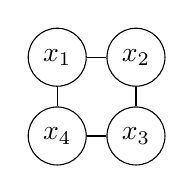
\begin{tikzpicture}[main/.style = {draw, circle}] 
	\node[main] (1) {$x_1$}; 
	\node[main] (2) [right of=1] {$x_2$}; 
	\node[main] (3) [below of=1] {$x_4$}; 
	\node[main] (4) [below of=2] {$x_3$}; 
	\draw[-] (1) -- (2);
	\draw[-] (4) -- (3);
	\draw[-] (1) -- (3);
	\draw[-] (2) -- (4);
\end{tikzpicture}
\caption{Sample UGM}
\label{fig:global-not-fact}		
\end{marginfigure}
We see this through a counter example. Consider the UGM in Figure \ref{fig:global-not-fact}, for the probability distribution $P(x_1, x_2, x_3, x_4)$ such that $P(x_1, x_2, x_3, x_4) = \frac{1}{8}$ when $x_1, x_2, x_3, x_4$ can take values from \\\noindent$\{0000, 1000, 1100, 1110, 1111, 0111, 0011, 0001\}$ else $0$. It can be manually checked that all 4 Global-CIs hold in the graph, for example $x_1 \ind x_3 | x_2, x_4$. Now consider the factors in the edges as $\psi(x_i, x_j)$. These will be positive, but that cannot represent the probability for $x_1, x_2, x_3, x_4 = 0101$. \\
Also, it is trivial to see that
\begin{equation}
	\text{Global-CI} \implies \text{Local-CI}
\end{equation}
But again through a counter example, we will show that the converse doesn't hold, i.e
\begin{equation}
	 \text{Local-CI} \nimplies \text{Global-CI}
\end{equation}
\begin{marginfigure}
	\centering
	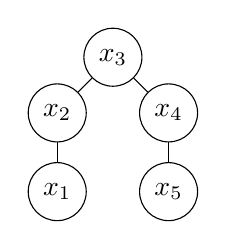
\begin{tikzpicture}[main/.style = {draw, circle}] 
		\node[main] (3) {$x_3$}; 
		\node[main] (4) [below right of=3] {$x_4$}; 
		\node[main] (2) [below left of=3] {$x_2$}; 
		\node[main] (5) [below of=4] {$x_5$}; 
		\node[main] (1) [below of=2] {$x_1$}; 
		\draw[-] (3) -- (2);
		\draw[-] (4) -- (3);
		\draw[-] (1) -- (2);
		\draw[-] (4) -- (5);
	\end{tikzpicture}
	\caption{Sample UGM}
	\label{fig:local-not-global}		
\end{marginfigure}
Consider a distribution over 5 binary variables $P(x_1, \cdots, x_5)$ where $x_1 = x_2, x_4 = x_5$ and $x_3 = x_2 \land x_4$. Consider $G$ as in Figure \ref{fig:local-not-global}. Notice that all 5 Local-CIs hold in the graph, for example $x_1 \ind \{x_3, x_4, x_5\} | x_2$. But notice that the graph also tells us that $x_2 \ind x_4 | x_3$, but this is not present in the distribution $P$. \\
We also notice that
\begin{equation}
	\text{Local-CI} \implies \text{Pairwise-CI}
\end{equation}
But again through a counter example, we show that the converse doesn't hold, i.e
\begin{equation}
 \text{Pairwise-CI}\nimplies 	\text{Local-CI}
\end{equation}
\begin{marginfigure}
	\centering
	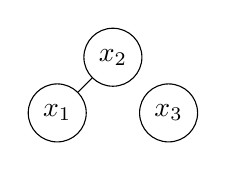
\begin{tikzpicture}[main/.style = {draw, circle}] 
		\node[main] (2) {$x_2$}; 
		\node[main] (1) [below left of=2] {$x_1$}; 
		\node[main] (3) [below right of=2] {$x_3$}; 
		\draw[-] (1) -- (2);
	\end{tikzpicture}
	\caption{Sample UGM}
	\label{fig:pairwise-not-local}		
\end{marginfigure}
Consider $P(x_1, x_2, x_3)$ defined over 3 binary variables such that $P(x_1,x_2,x_3) = \frac{1}{2}$ if $x_1=x_2=x_3$ and $0$ else. Let $G$ be as in Figure \ref{fig:pairwise-not-local}. See that both the Pairwise-CIs, i.e $x_1 \ind x_3 | x_2$ and $x_2 \ind x_3 | x_1$ hold in the graph, but the local CI $x_1 \ind x_3$ doesn't hold. \\
We have made a lot of statements about converses not holding in arbitrary distributions, but the natural question to arise is, can we find distributions where all the relations hold? The answer is yes, and is shown by the following theorem, also called the \textit{fundamental theorem of random fields} - 
\begin{thm}[Hammerseley Clifford Theorem]
If a positive distribution $P(x_1, \cdots x_n)$ confirms to the Pairwise-CIs of a UDGM $G$, then it can be factorized as per the cliques $C$ of $G$ as
\marginnote{A distribution $P(\mathbf x)$ is positive, if $P(\mathbf x) > 0 \; \forall \;\mathbf x$.}
\begin{equation}
	P(x_1, \cdots, x_n) \propto \prod_{C \in G} \psi_C(\mathbf{y}_C)
\end{equation}	
\end{thm}
\begin{proof}
Skipped.
\end{proof}
Thus, in summary, for any arbitrary distribution $P$ and UGM $H$,
\begin{equation}
	\begin{split}
	&\text{Factorize}(P, H) \implies \text{Global-CI}(P, H)\implies \\&\text{Local-CI}(P, H)\implies \text{Pairwise-CI}(P, H)
	\end{split}
\end{equation}
and if $P$ is positive, then
\begin{equation}
	\text{Pairwise-CI}(P, H) \implies \text{Factorize}(P, H)
\end{equation}
Hence, for a positive distribution, all three types of CIs are \textit{equivalent}.
\subsection{Minimal Construction}
The question to answer is, given a positive distribution $P(x_1, \cdots, x_n)$ as an oracle $\mathscr{O}$ to which we can ask the query - is $X\ind Y|Z$ and get a boolean answer, we need to draw a minimal and correct UGM $G$ to represent $P$. \\
Denote $V = \{x_1, x_2, \cdots, x_n\}$ as the set of all variables. We see that there are two methods to draw the UGM - 
\begin{enumerate}
	\item \textit{Using Pairwise-CIs:} For each pair of vertices $(x_i, x_j)$, if $x_i \ind x_j | V - \{x_i, x_j\}$ in $P$, add an edge between $x_i$ and $x_j$ in $G$.
	\item \textit{Using Local-CIs:} For each vector $x_i$, find the smallest subset $U$ such that $x_i \ind V - U - \{x_i\}|U$ in $P$. Then, add $U$ to $\mathcal{N}(x_i)$ in $P$.
\end{enumerate}
\begin{exmp}
	To be added.
\end{exmp}
We had seen Markov Blankets before, but we re-define them in terms of a UGM.
\begin{defn}[Markov Blanket]
The Markov Blanket (MB) of a variable $x_i$ is the smallest subset of variables $V$ that makes $x_i$ conditionally independent of others given the MB, i.e
\begin{equation}
x_i \ind V - MB(x_i) - \{x_i\} | MB(x_i)
\end{equation}
\end{defn}
\begin{thm}
The MB of a variable is always unique for a positive distribution.
\end{thm}
\begin{proof}
We will prove the following by contradiction. Let $x_i \in V$ and $M_1, M_2$ be two MBs. Let $\alpha = M_1 - M_2$ and $\beta = M_2 - M_1$, $M = M_1 \cap M_2$, $W = V - (M_1 \cup M_2)$. Note that, by definition, $x_i \ind V-M_2|M_2$ and $x_i \ind V-M_1|M_1$. Using this, we can write
\[x_i \ind W, \alpha|M, \beta \quad x_i \ind W, \beta|M,\alpha\]
For positive distributions, using intersection property, we can write
\[x_i \ind W, \alpha, \beta | M\]
This implies that $M$ is also a MB, but that is a contradiction since $M_1$ and $M_2$ were supposed to be minimal. Hence, the MB is unique.
\end{proof}
\marginnote{Interesetingly, UGMs were initially used to model interactions of atoms in gases and solids in 1800. A few other places where they are used are in 
\begin{enumerate}
	\item Markov Random Fields - Image Segmentation
	\item Conditional Random Fields - Information Extraction
	\item Social Networks
	\item Bio-informatics - Annotating active sites in proteins	 
\end{enumerate}
}
\begin{defn}[Immorality]
In a directed acyclic graph, the structure of the form $x \to y \leftarrow z$ is an immorality provided there is no edge between $x$ and $z$.
\end{defn}
With this, we can restate the equivalence of BNs - \\
\textit{Two BNs $\mathcal G_1$ and $\mathcal G_2$ are equivalent \textbf{iff} they have the same skeleton structure and the same set of immoralities}.
\subsection{Conversion to and from Bayesian Networks}
\begin{thm}
In a Bayesian Network $\mathcal G$, the Markov Blanket of a variable $x_i$ is given as
\begin{equation}
	MB(x_i) = \text{Pa}(x_i) \cup \text{Ch}(x_i) \cup \text{Sp}(x_i)
\end{equation}
where $\text{Pa}(x_i)$, $\text{Ch}(x_i)$ and $\text{Sp}(x_i)$ denote the parents, children and spouses (unmarried shared parent) of the children of $x_i$ (if exists).
\end{thm}
\begin{proof}
Only a flavor of the proof is provided. We have seen moralization of the Bayesian Network $\mathcal{G}$, and when we get $\mathcal{G}^M$ (i.e the moralized graph), notice that removing the parents, children and spouses disconnects the node from the graph.
\end{proof}
\begin{marginfigure}
	\centering
	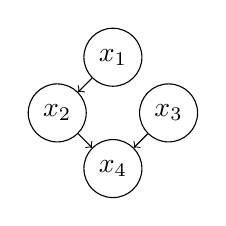
\begin{tikzpicture}[main/.style = {draw, circle}] 
		\node[main] (4) {$x_4$}; 
		\node[main] (2) [above left of=4] {$x_2$}; 
		\node[main] (3) [above right of=4] {$x_3$}; 
		\node[main] (1) [above right of=2] {$x_1$}; 
		\draw[->] (1) -- (2);
		\draw[->] (2) -- (4);
		\draw[->] (3) -- (4);
	\end{tikzpicture}
	\caption{Sample BN}
	\label{fig:bn-spouse-example}		
\end{marginfigure}
For example, in Figure \ref{fig:bn-spouse-example}, the MB of $x_2$ is given as
\[MB(x_2) = \{x_4\} \cup \{x_1\} \cup \{x_3\}\]
\begin{thm}
A Bayesian Network will have a perfect MRF if it has no immoralities.
\end{thm}
\begin{proof}
Skipped.
\end{proof}
We can ask the reverse question too. What condition should be posed on the MRF to have a perfect BN?
\begin{defn}[Chordal Graph]
A cordal graph is a simple graph in which every graph cycle of length four or greater has a cycle chord. 
\end{defn}
With this, we can state that
\begin{thm}
An MRF can be perfectly converted to a BN if and only if it is chordal.
\end{thm}
\begin{proof}
	Skipped.
\end{proof}